% Global Pipeline Architecture Diagram (English, CVPR/WACV style — exact column geometry, zero overlap)
\documentclass[tikz,border=3pt]{standalone}
\usepackage{fontspec}
\usepackage{amsmath,amssymb}
\setmainfont{DejaVu Serif}
\usetikzlibrary{positioning,fit,calc,arrows.meta,backgrounds}

\definecolor{cInk}{HTML}{1F2937}
\definecolor{cInkSoft}{HTML}{64748B}
\definecolor{cIn}{HTML}{F1F5F9}
\definecolor{cBack}{HTML}{E0F2FE}
\definecolor{cNeck}{HTML}{EEF2FF}
\definecolor{cNeckBorder}{HTML}{2563EB}
\definecolor{cGau}{HTML}{FFF3E0}
\definecolor{cGauBorder}{HTML}{C2410C}
\definecolor{cId}{HTML}{E6F4EA}
\definecolor{cIdBorder}{HTML}{0F766E}
\definecolor{cTrain}{HTML}{F5F3FF}
\definecolor{cTrainBorder}{HTML}{6D28D9}
\definecolor{cOut}{HTML}{F8FAFC}

\begin{document}
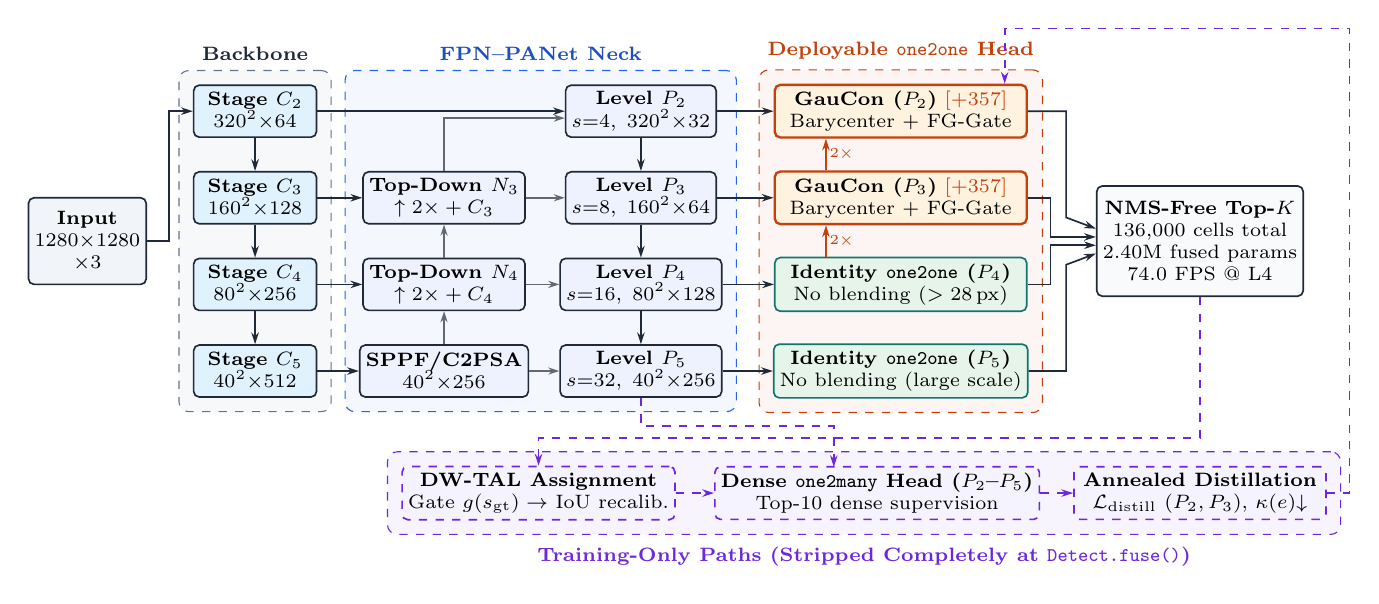
\begin{tikzpicture}[
  x=1cm, y=1cm,
  font=\scriptsize,
  blk/.style={draw=cInk, fill=#1, semithick, rounded corners=2pt,
              align=center, inner sep=2.2pt, minimum height=6.6mm},
  gblk/.style={draw=cGauBorder, fill=cGau, line width=0.85pt, rounded corners=2pt,
               align=center, inner sep=2.2pt, minimum height=6.6mm},
  iblk/.style={draw=cIdBorder, fill=cId, semithick, rounded corners=2pt,
               align=center, inner sep=2.2pt, minimum height=6.6mm},
  tblk/.style={draw=cTrainBorder, dashed, fill=cTrain, semithick, rounded corners=2pt,
               align=center, inner sep=2.2pt, minimum height=6.6mm},
  arr/.style={-{Stealth[length=1.5mm,width=0.95mm]}, cInk, semithick},
  darr/.style={-{Stealth[length=1.4mm,width=0.90mm]}, cInk!70, semithick},
  tarr/.style={-{Stealth[length=1.5mm,width=0.95mm]}, cTrainBorder, dashed, semithick},
  zone/.style={draw=#1, dashed, rounded corners=3.5pt, fill=#1!5!white, inner sep=5pt},
  zlbl/.style={font=\scriptsize\bfseries, text=#1},
]

% Column 0: Input (x=0.72, span [0.0..1.44])
\node[blk=cIn, minimum width=1.44cm, minimum height=11mm] (img) at (0.72, 2.55)
  {\textbf{Input}\\$1280{\times}1280$\\$\times 3$};

% Column 1: Backbone C2..C5 (x=2.85, span [2.07..3.63])
\node[blk=cBack, minimum width=1.56cm] (c2) at (2.85, 4.20) {\textbf{Stage $C_2$}\\$320^2{\times}64$};
\node[blk=cBack, minimum width=1.56cm] (c3) at (2.85, 3.10) {\textbf{Stage $C_3$}\\$160^2{\times}128$};
\node[blk=cBack, minimum width=1.56cm] (c4) at (2.85, 2.00) {\textbf{Stage $C_4$}\\$80^2{\times}256$};
\node[blk=cBack, minimum width=1.56cm] (c5) at (2.85, 0.90) {\textbf{Stage $C_5$}\\$40^2{\times}512$};

\draw[arr] (img.east) -- (1.76, 2.55) |- (c2.west);
\draw[arr] (c2.south) -- (c3.north);
\draw[arr] (c3.south) -- (c4.north);
\draw[arr] (c4.south) -- (c5.north);

% Column 2 & 3: FPN-PANet Neck (x=5.25 & x=7.75, span [4.35..8.68])
\node[blk=cNeck, minimum width=1.80cm] (td5) at (5.25, 0.90) {\textbf{SPPF/C2PSA}\\$40^2{\times}256$};
\node[blk=cNeck, minimum width=1.80cm] (td4) at (5.25, 2.00) {\textbf{Top-Down $N_4$}\\$\uparrow 2{\times} + C_4$};
\node[blk=cNeck, minimum width=1.80cm] (td3) at (5.25, 3.10) {\textbf{Top-Down $N_3$}\\$\uparrow 2{\times} + C_3$};

\node[blk=cNeck, minimum width=1.86cm] (p2)  at (7.75, 4.20) {\textbf{Level $P_2$}\\$s{=}4,\; 320^2{\times}32$};
\node[blk=cNeck, minimum width=1.86cm] (p3)  at (7.75, 3.10) {\textbf{Level $P_3$}\\$s{=}8,\; 160^2{\times}64$};
\node[blk=cNeck, minimum width=1.86cm] (p4)  at (7.75, 2.00) {\textbf{Level $P_4$}\\$s{=}16,\; 80^2{\times}128$};
\node[blk=cNeck, minimum width=1.86cm] (p5)  at (7.75, 0.90) {\textbf{Level $P_5$}\\$s{=}32,\; 40^2{\times}256$};

\draw[arr] (c5.east) -- (td5.west);
\draw[arr] (c4.east) -- (td4.west);
\draw[arr] (c3.east) -- (td3.west);
\draw[arr] (c2.east) -- (p2.west);

\draw[darr] (td5.north) -- (td4.south);
\draw[darr] (td4.north) -- (td3.south);
\draw[darr] (td3.north) |- ([yshift=-2.5pt]p2.west);

\draw[arr] (p2.south) -- (p3.north);
\draw[arr] (p3.south) -- (p4.north);
\draw[arr] (p4.south) -- (p5.north);
\draw[darr] (td3.east) -- (p3.west);
\draw[darr] (td4.east) -- (p4.west);
\draw[darr] (td5.east) -- (p5.west);

% Column 4: Deployable one2one Head (x=11.05, span [9.45..12.65])
\node[gblk, minimum width=3.20cm] (gc2) at (11.05, 4.20)
  {\textbf{GauCon ($P_2$)} \textcolor{cGauBorder}{$[+357]$}\\Barycenter + FG-Gate};
\node[gblk, minimum width=3.20cm] (gc3) at (11.05, 3.10)
  {\textbf{GauCon ($P_3$)} \textcolor{cGauBorder}{$[+357]$}\\Barycenter + FG-Gate};
\node[iblk, minimum width=3.20cm] (id4) at (11.05, 2.00)
  {\textbf{Identity \texttt{one2one} ($P_4$)}\\No blending ($>28$\,px)};
\node[iblk, minimum width=3.20cm] (id5) at (11.05, 0.90)
  {\textbf{Identity \texttt{one2one} ($P_5$)}\\No blending (large scale)};

\draw[arr] (p2.east) -- (gc2.west);
\draw[arr] (p3.east) -- (gc3.west);
\draw[arr] (p4.east) -- (id4.west);
\draw[arr] (p5.east) -- (id5.west);

\draw[arr, draw=cGauBorder] ([xshift=-0.95cm]gc3.north) -- node[right, font=\tiny, text=cGauBorder, inner sep=1pt]{$2{\times}$} ([xshift=-0.95cm]gc2.south);
\draw[arr, draw=cGauBorder] ([xshift=-0.95cm]id4.north) -- node[right, font=\tiny, text=cGauBorder, inner sep=1pt]{$2{\times}$} ([xshift=-0.95cm]gc3.south);

% Column 5: NMS-Free Output (x=14.85, span [13.62..16.08], 0.97 cm clear from Col 4!)
\node[blk=cOut, minimum width=2.45cm, minimum height=14mm] (out) at (14.85, 2.55)
  {\textbf{NMS-Free Top-$K$}\\$136{,}000$ cells total\\$2.40$M fused params\\$74.0$ FPS @ L4};

\draw[arr] (gc2.east) -| (13.15, 2.85) -- ([yshift=4.5pt]out.west);
\draw[arr] (gc3.east) -- (12.95, 3.10) |- ([yshift=1.5pt]out.west);
\draw[arr] (id4.east) -- (12.95, 2.00) |- ([yshift=-1.5pt]out.west);
\draw[arr] (id5.east) -| (13.15, 2.25) -- ([yshift=-4.5pt]out.west);

% Bottom Row: Training-Only Supervision (y=-0.65, below all inference layers)
\node[tblk, minimum width=3.20cm] (dwtal) at (6.45, -0.65)
  {\textbf{DW-TAL Assignment}\\Gate $g(s_{\mathrm{gt}}) \to$ IoU recalib.};
\node[tblk, minimum width=3.55cm] (o2m) at (10.75, -0.65)
  {\textbf{Dense \texttt{one2many} Head ($P_2\text{--}P_5$)}\\Top-$10$ dense supervision};
\node[tblk, minimum width=3.20cm] (dist) at (14.85, -0.65)
  {\textbf{Annealed Distillation}\\$\mathcal{L}_{\mathrm{distill}}$ ($P_2,P_3$), $\kappa(e){\downarrow}$};

\begin{scope}[on background layer]
  \node[zone=cInkSoft, fit=(c2)(c3)(c4)(c5), label={[zlbl=cInk]above:{Backbone}}] (zb) {};
  \node[zone=cNeckBorder, fit=(td5)(td4)(td3)(p2)(p3)(p4)(p5), label={[zlbl=cNeckBorder!80!black]above:{FPN--PANet Neck}}] (zn) {};
  \node[zone=cGauBorder, fit=(gc2)(gc3)(id4)(id5), label={[zlbl=cGauBorder]above:{Deployable \texttt{one2one} Head}}] (zh) {};
  \node[zone=cTrainBorder, fit=(dwtal)(o2m)(dist),
        label={[zlbl=cTrainBorder, yshift=-1pt]below:{Training-Only Paths (Stripped Completely at \texttt{Detect.fuse()})}}] (zt) {};
\end{scope}

% Orthogonal purple training arrows routed COMPLETELY outside zone headers
\draw[tarr] (p5.south) -- (7.75, 0.20) -| (10.20, -0.32);
\draw[tarr] (dwtal.east) -- (o2m.west);
\draw[tarr] (o2m.east) -- (dist.west);
\draw[tarr] (out.south) -- (14.85, 0.05) -| (dwtal.north);
% Distillation feedback loops cleanly over the top right clear of "Deployable one2one Head"
\draw[tarr] (dist.east) -- (16.75, -0.65) -- (16.75, 5.25) -| ([xshift=1.32cm]gc2.north);

\end{tikzpicture}
\end{document}